\subsection{ Databse Description}
This section describes the data base which will be used by the Ev3 Robot Controller program. The database consists of a repository of xml files that hold the information on the 
graphical representation of the map as shown in the GUI. The repository will hold the xml files which are exported by the user. The location xml files which the user will be importing will vary and wil not be stored by the program, it will simply be converted to an object that will replace the current map on the GUI. 
\subsection{Data Structures}
The data structure is represented by an ER diagram below. Note that the GUI map entity has no ujnique identifier. This is because the GUI map will be in constant state of change and only needs to be snapshotted on the export command.
\begin{figure}
    \centering
    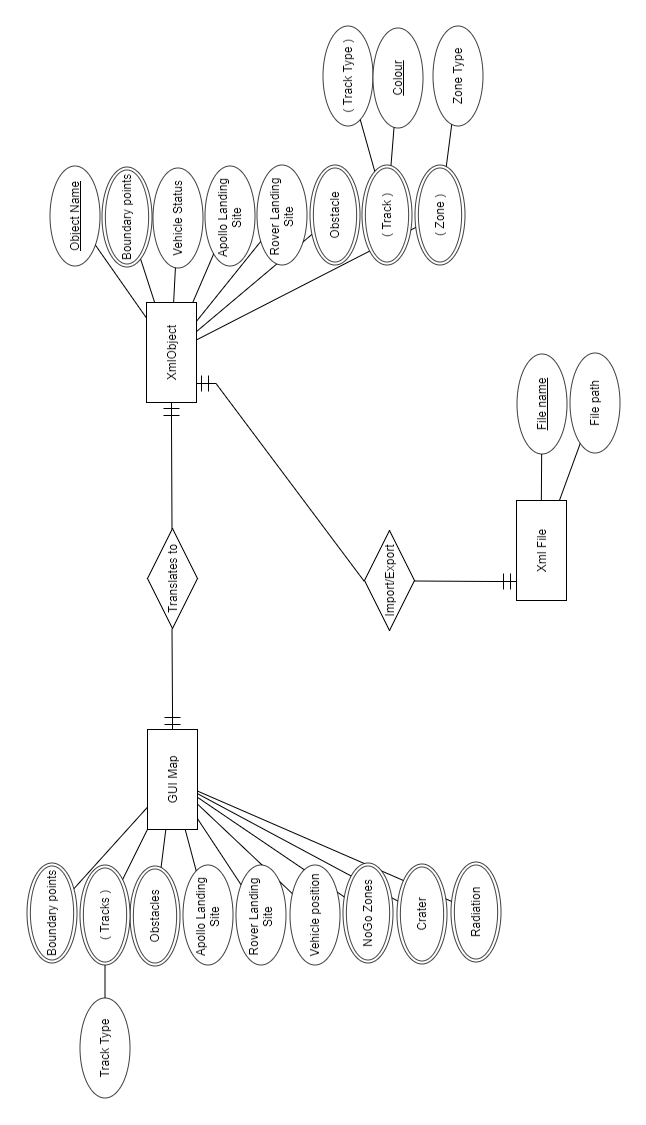
\includegraphics[width=0.9\textwidth] {erd.png}
    \caption{\label{fig:erd}Database ER Model}
\end{figure}


